\documentclass[aspect=169]{beamer}
\usepackage{graphicx}
\usepackage{tikz}
\usepackage[utf8]{inputenc}

\begin{document}
\begin{frame}<presentation>[label=FrameGrilla2x2]
  \frametitle{Grilla 2x2}

  \resizebox{\textwidth}{!}{ % GNUPLOT: LaTeX picture with Postscript
\begingroup
  \makeatletter
  \providecommand\color[2][]{%
    \GenericError{(gnuplot) \space\space\space\@spaces}{%
      Package color not loaded in conjunction with
      terminal option `colourtext'%
    }{See the gnuplot documentation for explanation.%
    }{Either use 'blacktext' in gnuplot or load the package
      color.sty in LaTeX.}%
    \renewcommand\color[2][]{}%
  }%
  \providecommand\includegraphics[2][]{%
    \GenericError{(gnuplot) \space\space\space\@spaces}{%
      Package graphicx or graphics not loaded%
    }{See the gnuplot documentation for explanation.%
    }{The gnuplot epslatex terminal needs graphicx.sty or graphics.sty.}%
    \renewcommand\includegraphics[2][]{}%
  }%
  \providecommand\rotatebox[2]{#2}%
  \@ifundefined{ifGPcolor}{%
    \newif\ifGPcolor
    \GPcolorfalse
  }{}%
  \@ifundefined{ifGPblacktext}{%
    \newif\ifGPblacktext
    \GPblacktexttrue
  }{}%
  % define a \g@addto@macro without @ in the name:
  \let\gplgaddtomacro\g@addto@macro
  % define empty templates for all commands taking text:
  \gdef\gplbacktext{}%
  \gdef\gplfronttext{}%
  \makeatother
  \ifGPblacktext
    % no textcolor at all
    \def\colorrgb#1{}%
    \def\colorgray#1{}%
  \else
    % gray or color?
    \ifGPcolor
      \def\colorrgb#1{\color[rgb]{#1}}%
      \def\colorgray#1{\color[gray]{#1}}%
      \expandafter\def\csname LTw\endcsname{\color{white}}%
      \expandafter\def\csname LTb\endcsname{\color{black}}%
      \expandafter\def\csname LTa\endcsname{\color{black}}%
      \expandafter\def\csname LT0\endcsname{\color[rgb]{1,0,0}}%
      \expandafter\def\csname LT1\endcsname{\color[rgb]{0,1,0}}%
      \expandafter\def\csname LT2\endcsname{\color[rgb]{0,0,1}}%
      \expandafter\def\csname LT3\endcsname{\color[rgb]{1,0,1}}%
      \expandafter\def\csname LT4\endcsname{\color[rgb]{0,1,1}}%
      \expandafter\def\csname LT5\endcsname{\color[rgb]{1,1,0}}%
      \expandafter\def\csname LT6\endcsname{\color[rgb]{0,0,0}}%
      \expandafter\def\csname LT7\endcsname{\color[rgb]{1,0.3,0}}%
      \expandafter\def\csname LT8\endcsname{\color[rgb]{0.5,0.5,0.5}}%
    \else
      % gray
      \def\colorrgb#1{\color{black}}%
      \def\colorgray#1{\color[gray]{#1}}%
      \expandafter\def\csname LTw\endcsname{\color{white}}%
      \expandafter\def\csname LTb\endcsname{\color{black}}%
      \expandafter\def\csname LTa\endcsname{\color{black}}%
      \expandafter\def\csname LT0\endcsname{\color{black}}%
      \expandafter\def\csname LT1\endcsname{\color{black}}%
      \expandafter\def\csname LT2\endcsname{\color{black}}%
      \expandafter\def\csname LT3\endcsname{\color{black}}%
      \expandafter\def\csname LT4\endcsname{\color{black}}%
      \expandafter\def\csname LT5\endcsname{\color{black}}%
      \expandafter\def\csname LT6\endcsname{\color{black}}%
      \expandafter\def\csname LT7\endcsname{\color{black}}%
      \expandafter\def\csname LT8\endcsname{\color{black}}%
    \fi
  \fi
    \setlength{\unitlength}{0.0500bp}%
    \ifx\gptboxheight\undefined%
      \newlength{\gptboxheight}%
      \newlength{\gptboxwidth}%
      \newsavebox{\gptboxtext}%
    \fi%
    \setlength{\fboxrule}{0.5pt}%
    \setlength{\fboxsep}{1pt}%
\begin{picture}(7200.00,5040.00)%
    \gplgaddtomacro\gplbacktext{%
      \csname LTb\endcsname%%
      \put(1078,440){\makebox(0,0)[r]{\strut{}$-0.05$}}%
      \put(1078,834){\makebox(0,0)[r]{\strut{}$0$}}%
      \put(1078,1228){\makebox(0,0)[r]{\strut{}$0.05$}}%
      \put(1078,1622){\makebox(0,0)[r]{\strut{}$0.1$}}%
      \put(1078,2016){\makebox(0,0)[r]{\strut{}$0.15$}}%
      \put(1078,2410){\makebox(0,0)[r]{\strut{}$0.2$}}%
      \put(1078,2803){\makebox(0,0)[r]{\strut{}$0.25$}}%
      \put(1078,3197){\makebox(0,0)[r]{\strut{}$0.3$}}%
      \put(1078,3591){\makebox(0,0)[r]{\strut{}$0.35$}}%
      \put(1078,3985){\makebox(0,0)[r]{\strut{}$0.4$}}%
      \put(1078,4379){\makebox(0,0)[r]{\strut{}$0.45$}}%
      \put(1210,220){\makebox(0,0){\strut{}$0$}}%
      \put(2142,220){\makebox(0,0){\strut{}$1$}}%
      \put(3074,220){\makebox(0,0){\strut{}$2$}}%
      \put(4007,220){\makebox(0,0){\strut{}$3$}}%
      \put(4939,220){\makebox(0,0){\strut{}$4$}}%
      \put(5871,220){\makebox(0,0){\strut{}$5$}}%
      \put(6803,220){\makebox(0,0){\strut{}$6$}}%
    }%
    \gplgaddtomacro\gplfronttext{%
      \csname LTb\endcsname%%
      \put(209,2409){\rotatebox{-270}{\makebox(0,0){\strut{}$ <E^2> - <E>^2  / kT^2 $}}}%
      \put(4006,4709){\makebox(0,0){\strut{}cálculos 2x2 vs teoria}}%
      \csname LTb\endcsname%%
      \put(5816,4206){\makebox(0,0)[r]{\strut{}2x2, 100000}}%
      \csname LTb\endcsname%%
      \put(5816,3986){\makebox(0,0)[r]{\strut{}2x2, 500000}}%
      \csname LTb\endcsname%%
      \put(5816,3766){\makebox(0,0)[r]{\strut{}2x2, 1000000}}%
      \csname LTb\endcsname%%
      \put(5816,3546){\makebox(0,0)[r]{\strut{}2x2, 5000000}}%
      \csname LTb\endcsname%%
      \put(5816,3326){\makebox(0,0)[r]{\strut{}resultado teorico}}%
    }%
    \gplbacktext
    \put(0,0){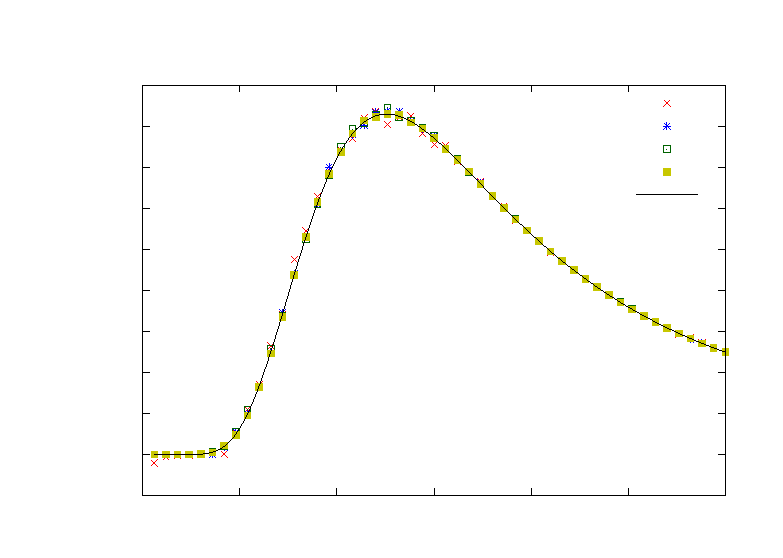
\includegraphics{scale_2x2}}%
    \gplfronttext
  \end{picture}%
\endgroup
 }

\end{frame}

\begin{frame}<presentation>[label=FrameGrilla16x16]
  \frametitle{Grilla 16x16}
  \resizebox{\textwidth}{!}{ % GNUPLOT: LaTeX picture with Postscript
\begingroup
  \makeatletter
  \providecommand\color[2][]{%
    \GenericError{(gnuplot) \space\space\space\@spaces}{%
      Package color not loaded in conjunction with
      terminal option `colourtext'%
    }{See the gnuplot documentation for explanation.%
    }{Either use 'blacktext' in gnuplot or load the package
      color.sty in LaTeX.}%
    \renewcommand\color[2][]{}%
  }%
  \providecommand\includegraphics[2][]{%
    \GenericError{(gnuplot) \space\space\space\@spaces}{%
      Package graphicx or graphics not loaded%
    }{See the gnuplot documentation for explanation.%
    }{The gnuplot epslatex terminal needs graphicx.sty or graphics.sty.}%
    \renewcommand\includegraphics[2][]{}%
  }%
  \providecommand\rotatebox[2]{#2}%
  \@ifundefined{ifGPcolor}{%
    \newif\ifGPcolor
    \GPcolorfalse
  }{}%
  \@ifundefined{ifGPblacktext}{%
    \newif\ifGPblacktext
    \GPblacktexttrue
  }{}%
  % define a \g@addto@macro without @ in the name:
  \let\gplgaddtomacro\g@addto@macro
  % define empty templates for all commands taking text:
  \gdef\gplbacktext{}%
  \gdef\gplfronttext{}%
  \makeatother
  \ifGPblacktext
    % no textcolor at all
    \def\colorrgb#1{}%
    \def\colorgray#1{}%
  \else
    % gray or color?
    \ifGPcolor
      \def\colorrgb#1{\color[rgb]{#1}}%
      \def\colorgray#1{\color[gray]{#1}}%
      \expandafter\def\csname LTw\endcsname{\color{white}}%
      \expandafter\def\csname LTb\endcsname{\color{black}}%
      \expandafter\def\csname LTa\endcsname{\color{black}}%
      \expandafter\def\csname LT0\endcsname{\color[rgb]{1,0,0}}%
      \expandafter\def\csname LT1\endcsname{\color[rgb]{0,1,0}}%
      \expandafter\def\csname LT2\endcsname{\color[rgb]{0,0,1}}%
      \expandafter\def\csname LT3\endcsname{\color[rgb]{1,0,1}}%
      \expandafter\def\csname LT4\endcsname{\color[rgb]{0,1,1}}%
      \expandafter\def\csname LT5\endcsname{\color[rgb]{1,1,0}}%
      \expandafter\def\csname LT6\endcsname{\color[rgb]{0,0,0}}%
      \expandafter\def\csname LT7\endcsname{\color[rgb]{1,0.3,0}}%
      \expandafter\def\csname LT8\endcsname{\color[rgb]{0.5,0.5,0.5}}%
    \else
      % gray
      \def\colorrgb#1{\color{black}}%
      \def\colorgray#1{\color[gray]{#1}}%
      \expandafter\def\csname LTw\endcsname{\color{white}}%
      \expandafter\def\csname LTb\endcsname{\color{black}}%
      \expandafter\def\csname LTa\endcsname{\color{black}}%
      \expandafter\def\csname LT0\endcsname{\color{black}}%
      \expandafter\def\csname LT1\endcsname{\color{black}}%
      \expandafter\def\csname LT2\endcsname{\color{black}}%
      \expandafter\def\csname LT3\endcsname{\color{black}}%
      \expandafter\def\csname LT4\endcsname{\color{black}}%
      \expandafter\def\csname LT5\endcsname{\color{black}}%
      \expandafter\def\csname LT6\endcsname{\color{black}}%
      \expandafter\def\csname LT7\endcsname{\color{black}}%
      \expandafter\def\csname LT8\endcsname{\color{black}}%
    \fi
  \fi
    \setlength{\unitlength}{0.0500bp}%
    \ifx\gptboxheight\undefined%
      \newlength{\gptboxheight}%
      \newlength{\gptboxwidth}%
      \newsavebox{\gptboxtext}%
    \fi%
    \setlength{\fboxrule}{0.5pt}%
    \setlength{\fboxsep}{1pt}%
\begin{picture}(7200.00,5040.00)%
    \gplgaddtomacro\gplbacktext{%
      \csname LTb\endcsname%%
      \put(1342,440){\makebox(0,0)[r]{\strut{}$-500000$}}%
      \put(1342,1003){\makebox(0,0)[r]{\strut{}$-400000$}}%
      \put(1342,1565){\makebox(0,0)[r]{\strut{}$-300000$}}%
      \put(1342,2128){\makebox(0,0)[r]{\strut{}$-200000$}}%
      \put(1342,2691){\makebox(0,0)[r]{\strut{}$-100000$}}%
      \put(1342,3254){\makebox(0,0)[r]{\strut{}$0$}}%
      \put(1342,3816){\makebox(0,0)[r]{\strut{}$100000$}}%
      \put(1342,4379){\makebox(0,0)[r]{\strut{}$200000$}}%
      \put(1474,220){\makebox(0,0){\strut{}$0$}}%
      \put(2362,220){\makebox(0,0){\strut{}$1$}}%
      \put(3250,220){\makebox(0,0){\strut{}$2$}}%
      \put(4139,220){\makebox(0,0){\strut{}$3$}}%
      \put(5027,220){\makebox(0,0){\strut{}$4$}}%
      \put(5915,220){\makebox(0,0){\strut{}$5$}}%
      \put(6803,220){\makebox(0,0){\strut{}$6$}}%
    }%
    \gplgaddtomacro\gplfronttext{%
      \csname LTb\endcsname%%
      \put(209,2409){\rotatebox{-270}{\makebox(0,0){\strut{}$ <E^2> - <E>^2  / kT^2 $}}}%
      \put(4138,4709){\makebox(0,0){\strut{}cálculos 16x16}}%
      \csname LTb\endcsname%%
      \put(5816,4206){\makebox(0,0)[r]{\strut{}16x16, 10000}}%
      \csname LTb\endcsname%%
      \put(5816,3986){\makebox(0,0)[r]{\strut{}16x16, 50000}}%
      \csname LTb\endcsname%%
      \put(5816,3766){\makebox(0,0)[r]{\strut{}16x16, 100000}}%
      \csname LTb\endcsname%%
      \put(5816,3546){\makebox(0,0)[r]{\strut{}16x16, 500000}}%
      \csname LTb\endcsname%%
      \put(5816,3326){\makebox(0,0)[r]{\strut{}16x16, 1000000}}%
      \csname LTb\endcsname%%
      \put(5816,3106){\makebox(0,0)[r]{\strut{}16x16, 5000000}}%
    }%
    \gplbacktext
    \put(0,0){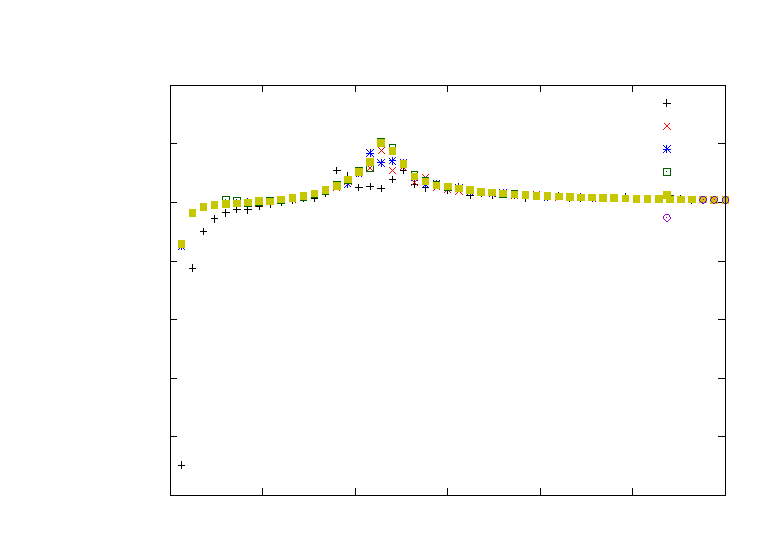
\includegraphics{scale_16x16}}%
    \gplfronttext
  \end{picture}%
\endgroup
 }
  
\end{frame}

\begin{frame}<presentation>[label=FrameMomentoMagnetico]
  \frametitle{Evolución del Momento Magnético}
  \resizebox{\textwidth}{!}{% GNUPLOT: LaTeX picture with Postscript
\begingroup
  \makeatletter
  \providecommand\color[2][]{%
    \GenericError{(gnuplot) \space\space\space\@spaces}{%
      Package color not loaded in conjunction with
      terminal option `colourtext'%
    }{See the gnuplot documentation for explanation.%
    }{Either use 'blacktext' in gnuplot or load the package
      color.sty in LaTeX.}%
    \renewcommand\color[2][]{}%
  }%
  \providecommand\includegraphics[2][]{%
    \GenericError{(gnuplot) \space\space\space\@spaces}{%
      Package graphicx or graphics not loaded%
    }{See the gnuplot documentation for explanation.%
    }{The gnuplot epslatex terminal needs graphicx.sty or graphics.sty.}%
    \renewcommand\includegraphics[2][]{}%
  }%
  \providecommand\rotatebox[2]{#2}%
  \@ifundefined{ifGPcolor}{%
    \newif\ifGPcolor
    \GPcolorfalse
  }{}%
  \@ifundefined{ifGPblacktext}{%
    \newif\ifGPblacktext
    \GPblacktexttrue
  }{}%
  % define a \g@addto@macro without @ in the name:
  \let\gplgaddtomacro\g@addto@macro
  % define empty templates for all commands taking text:
  \gdef\gplbacktext{}%
  \gdef\gplfronttext{}%
  \makeatother
  \ifGPblacktext
    % no textcolor at all
    \def\colorrgb#1{}%
    \def\colorgray#1{}%
  \else
    % gray or color?
    \ifGPcolor
      \def\colorrgb#1{\color[rgb]{#1}}%
      \def\colorgray#1{\color[gray]{#1}}%
      \expandafter\def\csname LTw\endcsname{\color{white}}%
      \expandafter\def\csname LTb\endcsname{\color{black}}%
      \expandafter\def\csname LTa\endcsname{\color{black}}%
      \expandafter\def\csname LT0\endcsname{\color[rgb]{1,0,0}}%
      \expandafter\def\csname LT1\endcsname{\color[rgb]{0,1,0}}%
      \expandafter\def\csname LT2\endcsname{\color[rgb]{0,0,1}}%
      \expandafter\def\csname LT3\endcsname{\color[rgb]{1,0,1}}%
      \expandafter\def\csname LT4\endcsname{\color[rgb]{0,1,1}}%
      \expandafter\def\csname LT5\endcsname{\color[rgb]{1,1,0}}%
      \expandafter\def\csname LT6\endcsname{\color[rgb]{0,0,0}}%
      \expandafter\def\csname LT7\endcsname{\color[rgb]{1,0.3,0}}%
      \expandafter\def\csname LT8\endcsname{\color[rgb]{0.5,0.5,0.5}}%
    \else
      % gray
      \def\colorrgb#1{\color{black}}%
      \def\colorgray#1{\color[gray]{#1}}%
      \expandafter\def\csname LTw\endcsname{\color{white}}%
      \expandafter\def\csname LTb\endcsname{\color{black}}%
      \expandafter\def\csname LTa\endcsname{\color{black}}%
      \expandafter\def\csname LT0\endcsname{\color{black}}%
      \expandafter\def\csname LT1\endcsname{\color{black}}%
      \expandafter\def\csname LT2\endcsname{\color{black}}%
      \expandafter\def\csname LT3\endcsname{\color{black}}%
      \expandafter\def\csname LT4\endcsname{\color{black}}%
      \expandafter\def\csname LT5\endcsname{\color{black}}%
      \expandafter\def\csname LT6\endcsname{\color{black}}%
      \expandafter\def\csname LT7\endcsname{\color{black}}%
      \expandafter\def\csname LT8\endcsname{\color{black}}%
    \fi
  \fi
    \setlength{\unitlength}{0.0500bp}%
    \ifx\gptboxheight\undefined%
      \newlength{\gptboxheight}%
      \newlength{\gptboxwidth}%
      \newsavebox{\gptboxtext}%
    \fi%
    \setlength{\fboxrule}{0.5pt}%
    \setlength{\fboxsep}{1pt}%
\begin{picture}(7200.00,5040.00)%
    \gplgaddtomacro\gplbacktext{%
      \csname LTb\endcsname%%
      \put(814,704){\makebox(0,0)[r]{\strut{}$0$}}%
      \put(814,1072){\makebox(0,0)[r]{\strut{}$0.1$}}%
      \put(814,1439){\makebox(0,0)[r]{\strut{}$0.2$}}%
      \put(814,1807){\makebox(0,0)[r]{\strut{}$0.3$}}%
      \put(814,2174){\makebox(0,0)[r]{\strut{}$0.4$}}%
      \put(814,2542){\makebox(0,0)[r]{\strut{}$0.5$}}%
      \put(814,2909){\makebox(0,0)[r]{\strut{}$0.6$}}%
      \put(814,3277){\makebox(0,0)[r]{\strut{}$0.7$}}%
      \put(814,3644){\makebox(0,0)[r]{\strut{}$0.8$}}%
      \put(814,4011){\makebox(0,0)[r]{\strut{}$0.9$}}%
      \put(814,4379){\makebox(0,0)[r]{\strut{}$1$}}%
      \put(946,484){\makebox(0,0){\strut{}$1$}}%
      \put(2117,484){\makebox(0,0){\strut{}$2$}}%
      \put(3289,484){\makebox(0,0){\strut{}$3$}}%
      \put(4460,484){\makebox(0,0){\strut{}$4$}}%
      \put(5632,484){\makebox(0,0){\strut{}$5$}}%
      \put(6803,484){\makebox(0,0){\strut{}$6$}}%
    }%
    \gplgaddtomacro\gplfronttext{%
      \csname LTb\endcsname%%
      \put(209,2541){\rotatebox{-270}{\makebox(0,0){\strut{}$||M||$}}}%
      \put(3874,154){\makebox(0,0){\strut{}$ T / T_0$}}%
      \put(3874,4709){\makebox(0,0){\strut{} resultados para 5M MCS }}%
      \put(5483,4206){\makebox(0,0){\strut{} tamaño de sistema }}%
      \csname LTb\endcsname%%
      \put(4955,3986){\makebox(0,0)[r]{\strut{}4x4}}%
      \csname LTb\endcsname%%
      \put(4955,3766){\makebox(0,0)[r]{\strut{}8x8}}%
      \csname LTb\endcsname%%
      \put(4955,3546){\makebox(0,0)[r]{\strut{}16x16}}%
    }%
    \gplbacktext
    \put(0,0){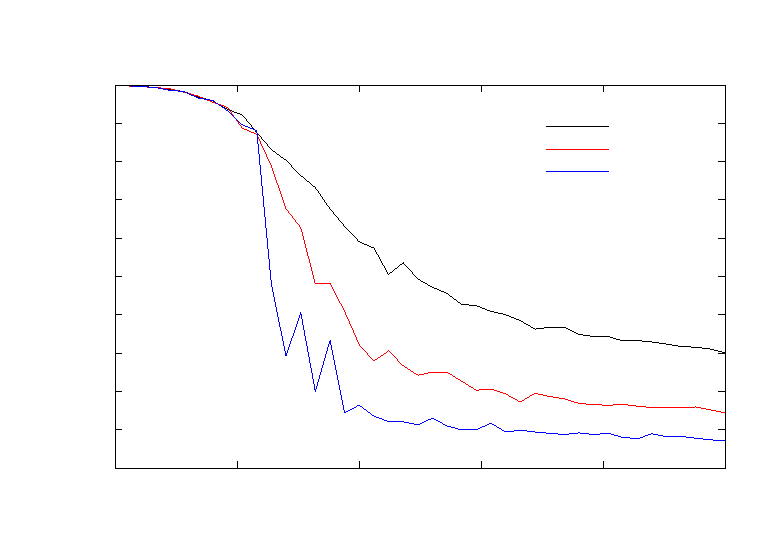
\includegraphics{scale_M_N}}%
    \gplfronttext
  \end{picture}%
\endgroup
}
\end{frame}

\begin{frame}<presentation>[label=FrameCalorEspecifico]
  \frametitle{Evolución del calor específico}
  \resizebox{\textwidth}{!}{% GNUPLOT: LaTeX picture with Postscript
\begingroup
  \makeatletter
  \providecommand\color[2][]{%
    \GenericError{(gnuplot) \space\space\space\@spaces}{%
      Package color not loaded in conjunction with
      terminal option `colourtext'%
    }{See the gnuplot documentation for explanation.%
    }{Either use 'blacktext' in gnuplot or load the package
      color.sty in LaTeX.}%
    \renewcommand\color[2][]{}%
  }%
  \providecommand\includegraphics[2][]{%
    \GenericError{(gnuplot) \space\space\space\@spaces}{%
      Package graphicx or graphics not loaded%
    }{See the gnuplot documentation for explanation.%
    }{The gnuplot epslatex terminal needs graphicx.sty or graphics.sty.}%
    \renewcommand\includegraphics[2][]{}%
  }%
  \providecommand\rotatebox[2]{#2}%
  \@ifundefined{ifGPcolor}{%
    \newif\ifGPcolor
    \GPcolorfalse
  }{}%
  \@ifundefined{ifGPblacktext}{%
    \newif\ifGPblacktext
    \GPblacktexttrue
  }{}%
  % define a \g@addto@macro without @ in the name:
  \let\gplgaddtomacro\g@addto@macro
  % define empty templates for all commands taking text:
  \gdef\gplbacktext{}%
  \gdef\gplfronttext{}%
  \makeatother
  \ifGPblacktext
    % no textcolor at all
    \def\colorrgb#1{}%
    \def\colorgray#1{}%
  \else
    % gray or color?
    \ifGPcolor
      \def\colorrgb#1{\color[rgb]{#1}}%
      \def\colorgray#1{\color[gray]{#1}}%
      \expandafter\def\csname LTw\endcsname{\color{white}}%
      \expandafter\def\csname LTb\endcsname{\color{black}}%
      \expandafter\def\csname LTa\endcsname{\color{black}}%
      \expandafter\def\csname LT0\endcsname{\color[rgb]{1,0,0}}%
      \expandafter\def\csname LT1\endcsname{\color[rgb]{0,1,0}}%
      \expandafter\def\csname LT2\endcsname{\color[rgb]{0,0,1}}%
      \expandafter\def\csname LT3\endcsname{\color[rgb]{1,0,1}}%
      \expandafter\def\csname LT4\endcsname{\color[rgb]{0,1,1}}%
      \expandafter\def\csname LT5\endcsname{\color[rgb]{1,1,0}}%
      \expandafter\def\csname LT6\endcsname{\color[rgb]{0,0,0}}%
      \expandafter\def\csname LT7\endcsname{\color[rgb]{1,0.3,0}}%
      \expandafter\def\csname LT8\endcsname{\color[rgb]{0.5,0.5,0.5}}%
    \else
      % gray
      \def\colorrgb#1{\color{black}}%
      \def\colorgray#1{\color[gray]{#1}}%
      \expandafter\def\csname LTw\endcsname{\color{white}}%
      \expandafter\def\csname LTb\endcsname{\color{black}}%
      \expandafter\def\csname LTa\endcsname{\color{black}}%
      \expandafter\def\csname LT0\endcsname{\color{black}}%
      \expandafter\def\csname LT1\endcsname{\color{black}}%
      \expandafter\def\csname LT2\endcsname{\color{black}}%
      \expandafter\def\csname LT3\endcsname{\color{black}}%
      \expandafter\def\csname LT4\endcsname{\color{black}}%
      \expandafter\def\csname LT5\endcsname{\color{black}}%
      \expandafter\def\csname LT6\endcsname{\color{black}}%
      \expandafter\def\csname LT7\endcsname{\color{black}}%
      \expandafter\def\csname LT8\endcsname{\color{black}}%
    \fi
  \fi
    \setlength{\unitlength}{0.0500bp}%
    \ifx\gptboxheight\undefined%
      \newlength{\gptboxheight}%
      \newlength{\gptboxwidth}%
      \newsavebox{\gptboxtext}%
    \fi%
    \setlength{\fboxrule}{0.5pt}%
    \setlength{\fboxsep}{1pt}%
\begin{picture}(7200.00,5040.00)%
    \gplgaddtomacro\gplbacktext{%
      \csname LTb\endcsname%%
      \put(814,704){\makebox(0,0)[r]{\strut{}$0$}}%
      \put(814,1229){\makebox(0,0)[r]{\strut{}$0.2$}}%
      \put(814,1754){\makebox(0,0)[r]{\strut{}$0.4$}}%
      \put(814,2279){\makebox(0,0)[r]{\strut{}$0.6$}}%
      \put(814,2804){\makebox(0,0)[r]{\strut{}$0.8$}}%
      \put(814,3329){\makebox(0,0)[r]{\strut{}$1$}}%
      \put(814,3854){\makebox(0,0)[r]{\strut{}$1.2$}}%
      \put(814,4379){\makebox(0,0)[r]{\strut{}$1.4$}}%
      \put(946,484){\makebox(0,0){\strut{}$1$}}%
      \put(2117,484){\makebox(0,0){\strut{}$2$}}%
      \put(3289,484){\makebox(0,0){\strut{}$3$}}%
      \put(4460,484){\makebox(0,0){\strut{}$4$}}%
      \put(5632,484){\makebox(0,0){\strut{}$5$}}%
      \put(6803,484){\makebox(0,0){\strut{}$6$}}%
    }%
    \gplgaddtomacro\gplfronttext{%
      \csname LTb\endcsname%%
      \put(209,2541){\rotatebox{-270}{\makebox(0,0){\strut{}$ <E^2> - <E>^2  / kT^2 $}}}%
      \put(3874,154){\makebox(0,0){\strut{}$ T / T_0$}}%
      \put(3874,4709){\makebox(0,0){\strut{} resultados para 5M MCS }}%
      \put(5483,4206){\makebox(0,0){\strut{} tamaño de sistema }}%
      \csname LTb\endcsname%%
      \put(4559,3986){\makebox(0,0)[r]{\strut{}4}}%
      \csname LTb\endcsname%%
      \put(4559,3766){\makebox(0,0)[r]{\strut{}8}}%
      \csname LTb\endcsname%%
      \put(4559,3546){\makebox(0,0)[r]{\strut{}16}}%
    }%
    \gplbacktext
    \put(0,0){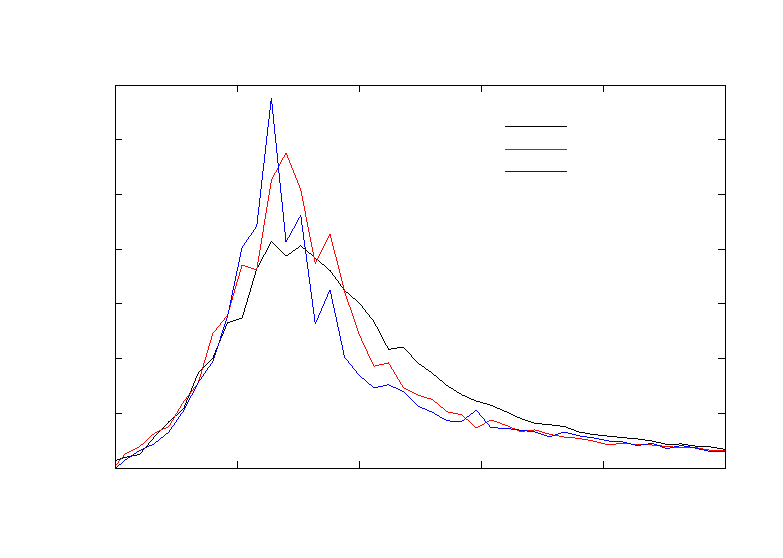
\includegraphics{scale_cv_N}}%
    \gplfronttext
  \end{picture}%
\endgroup
} 
\end{frame}
\end{document}
